\documentclass{article}
\usepackage[utf8]{inputenc}
%Pacchetto per le equazioni matematiche
\usepackage{amsmath}
%Pacchetto per i grafici
\usepackage{graphicx}

\title{Progetto Controlli 3A}
\author{
Luca Bartolomei\\
\texttt{0000825005}
\and
Federico Maria Macchiavelli\\
\texttt{0000825621}
\and
Mattia Innocenti\\
\texttt{0000825046}
\and
Andrea Proia\\
\texttt{0000825784}}

\date{Dicembre 2019}

\begin{document}

\maketitle

\section{Introduzione}

Progettazione di un controllore per un impianto idroelettrico, mediante l'utilizzo delle tecniche di controllo.

\section{Impianto idroelettrico}

L'impianto idroelettrico è modellato come sistema SISO avente due variabili di stato (la pressione  dell’acqua sul fondo del bacino ($x_1$) e la portata in uscita dal bacino ($x_2$ )). Le equazioni differenziali che modellano le variabili di stato sono di tipo non lineare:

$$
\dot{x}_1 = 0
$$

$$
\dot{x}_2 = -C_d u x_2 |x_2| -R_0 x_2 |x_2| + x_1
$$

L'uscita del sistema viene modellata secondo la formula:

$$
y=-\eta x_1 x_2
$$

\subsection{Significato fisico}

Il sistema modella la pressione sul fondo del bacino come costante, mentre la variazione nel tempo della portata nel fondo del bacino dipende da tre fattori:

\begin{itemize}
    \item Pressione sul fondo del bacino ($x_1$): Una pressione positiva contribuisce ad aumentare la portata nel fondo del bacino
    \item Perdite di carico nella condotta ($-R_0 x_2 |x_2|$): Si tratta dell'attrito tra la condotta e l'acqua, che contribuisce a diminuire la portata
    \item Valvola di controllo ($-C_d u x_2 |x_2|$): Consiste in una valvola che se opportunamente controllata permette di aumentare l'effetto di perdita di carico nella condotta.
\end{itemize}

L'uscita $y=-\eta x_1 x_2$ rappresenta la potenza elettrica generata dall'impianto. Viene calcolata come la potenza fluidica $x_1 x_2$ e moltiplicata per un coefficiente che indica l'efficienza di conversione tra energia meccanica e energia elettrica. Il segno negativo è dovuto al trasduttore utilizzato.

\subsection{Progettazione fisica del controllo}

Ragionando in termini di progettazione reale, il segnale ricevuto dal trasduttore di potenza sarà di tipo elettrico, il quale verrà letto da un circuito elettronico, il quale sarà realizzato mediante la rete regolatrice da noi progettata. 
Infine anche il segnale di controllo sarà di natura elettrica, quindi necessitiamo di un attuatore, per esempio un motore elettrico o un solenoide, magari con circuiteria aggiuntiva di potenza e di un sistema meccanico per l'interacciamento valvola-motore, per controllare la valvola, oppure sostituire una valvola con una elettro-valvola, avente attuatore già incluso.

\section{Specifiche}

L'azienda che ci ha assunto ha fornito delle specifiche sul sistema di controllo andremmo a progettare:

\begin{itemize}
    \item Errore a regime nullo ($e_{inf}=0$) per un gradino di ampiezza 30
    \item Sovraelongazione percentuale minore del 5\%
    \item Tempo di assestamento all'1\% minore di 0.3 sec
    \item Attenuazione dei rumori di misura di almeno 30 volte
    \item Margine di fase di almeno 45 gradi
\end{itemize}

Si aggiungono delle opzioni facoltative:
\begin{itemize}
    \item Aumento delle performance del sistema di controllo, modificando il tempo di assestamento all'1\% il quale dovrà essere minore di 0.033 sec
    \item Analisi delle performance del regolatore sul sistema non lineare in un intorno della coppia di equilibrio.
\end{itemize}

\section{Linearizzazione del sistema}

Per prima cosa linearizziamo il sistema idroelettrico in un sistema lineare. Per fare ciò utilizziamo la coppia di equilibrio fornita $x=(10,6), u=(\frac{\frac{x_1}{x_2 |x_2|}-R_0}{C_d})$:

Mediante la linearizzazione troviamo le quattro matrici $A,B,C,D$:

$$
A=
\begin{bmatrix}
    0 & 0\\
    1 & -3.333
\end{bmatrix}
B=
\begin{bmatrix}
    0\\
    -710.6115
\end{bmatrix}\\
C=
\begin{bmatrix}
    -3.6 & -6
\end{bmatrix}
D=0
$$

Da esse si ricava la funzione di trasferimento:

$$
G=\frac{4263.7 s}{s (s+3.333)}
$$

\subsection{Verifica delle prestazioni ad anello chiuso}

Analizziamo la rispsta al gradino del sistema senza regolatore in retroazione:

\begin{center}
    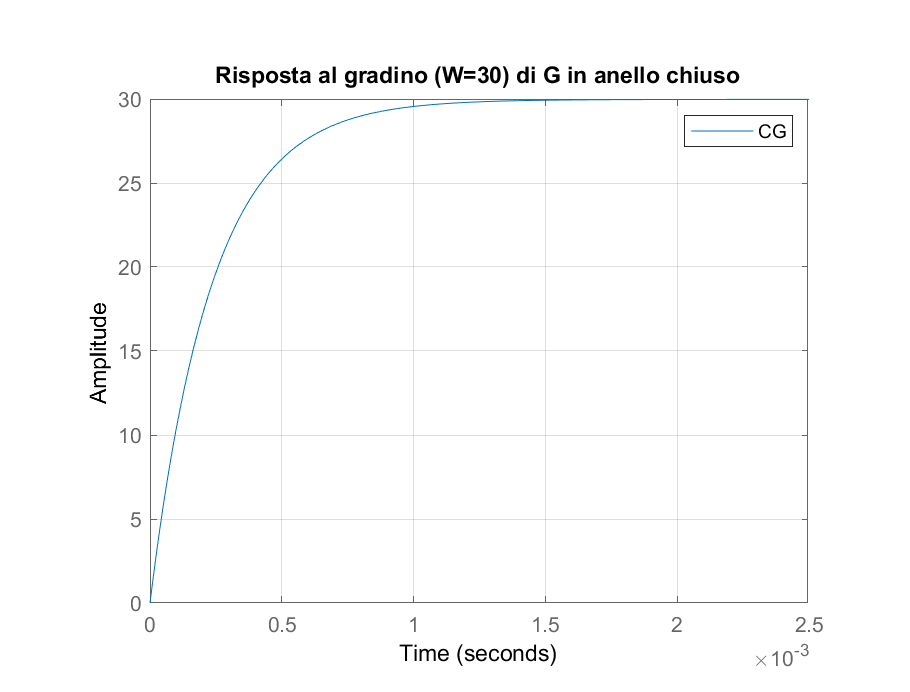
\includegraphics[scale=0.6]{figure1.eps}
\end{center}

Dalla figura possiamo evidenziare le sequenti performance:

\begin{itemize}
    \item Tempo di assestamento all'1\% molto basso, minore di 0.01 sec
    \item Sovraelongazione percentuale inferiore al 5%
\end{itemize}

Il sistema però non soddisfa alcune caratteristiche richeste:

\begin{itemize}
    \item Errore a regime non nullo (ma comunque basso visto l'alto guadagno del sistema in anello aperto)
    \item Attenuazione del rumore di misura quasi nullo
\end{itemize}

In conclusione abbiamo bisogno di un regolatore per risolvere le problematiche del sistema in retroazione.

\section{Progettazione del regolatore}

\subsection{Progettazione della rete regolatrice statica}

Per garantire un errore a regime nullo abbiamo bisogno di un regolatore statico:

$$
R_s(s)=\frac{1}{s}
$$

Il guadagno $\mu_s$ risulta libero e può essere usato successivamente se ci ritroveremmo in uno scenario A.

Proviamo a disegnare il diagramma di Bode per verificare in quale scenario ci siamo collocati.

\begin{center}
    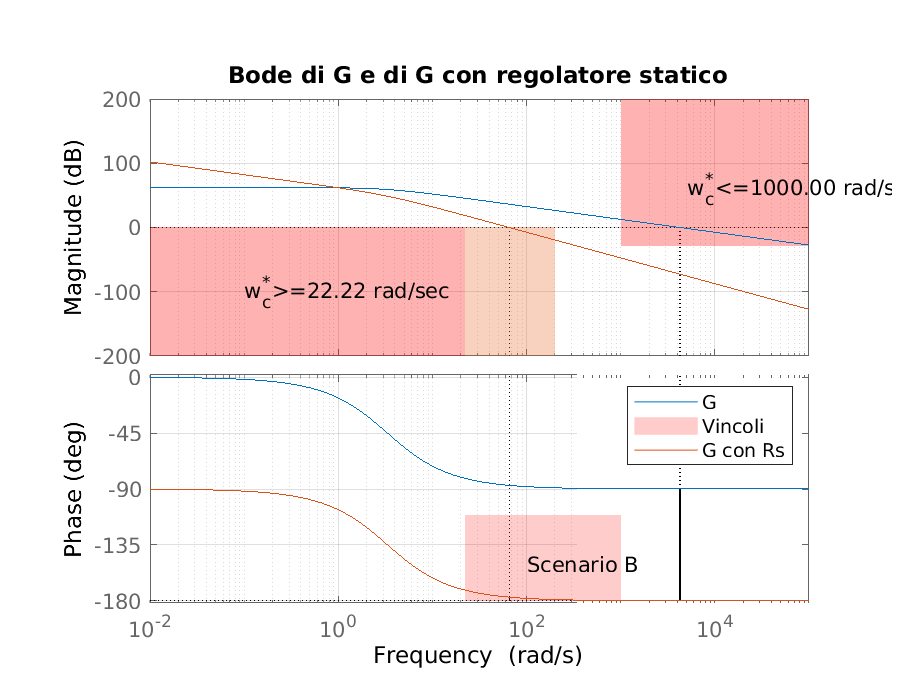
\includegraphics[scale=0.6]{figure2.eps}
\end{center}

Visto che il margine di fase risulta insufficiente per tutto l'intervallo di attraversamento, deduciamo che siamo caduti in uno scenario di tipo A.

\subsection{Progettazione della rete regolatrice dinamica}

Per ovviare allo scenario B, abbiamo bisogno di un regolatore dinamico formato da una rete anticipatrice.

$$
R_d(S)=\frac{1+\tau s}{1+\tau \alpha s}
$$

Il polo presente della rete anticipatrice è dovuto alla fisica realizzabilità della rete.

Rimane il problema di dove porre lo zero e il polo nel piano complesso:
\begin{itemize}
    \item Lo zero deve fornire un aumento di fase tale da superare il vincolo del margine di fase in almeno una parte del range di attraversamento
    \item Il polo deve essere collocato in alta frequenza (molto lontano dall'asse degli immaginari) per non disturbare l'effetto dello zero.
\end{itemize}

Potremmo utilizzare le formule di inversione per calcolare $\alpha$ e $\tau$. In questo caso abbiamo preferito l'utilizzo del luogo delle radici per il rispetto dei vincoli di sovraelongazione e di tempo di assestamento, mentre abbiamo osservato il diagramma di bode della funzione di trasferimento $G_e = R_s * G$ per calcolare il guadagno necessario per soddisfare il vincolo sull'attenuazione di misura.

\subsection{Attenuazione necessaria per il rumore di misura}

Utilizzando le funzioni di matlab e il diagramma di Bode, abbiamo calcolato il valore massimo di $\mu_d$, ancora libero in quanto non usato nel regolatore statico, per rispettare il vincolo di attenuazione di misura.

$$
    \mu_{d_B}=0.073446254984543
$$

\subsection{Vincolo di $\mu_d$ per la specifica di sovraelongazione}

Utilizzando il luogo delle radici siamo riusciti a calcolare il valore massimo di $\mu_d$


\end{document}

